\documentclass[a4paper,10pt,notitlepage]{scrartcl}

\usepackage[T1]{fontenc}
\usepackage[english]{babel}
\usepackage[utf8x]{inputenc}
\usepackage{setspace}
\usepackage{subfig}
\usepackage{textcomp}
\usepackage{graphicx}
\usepackage{fixltx2e}
\usepackage{multirow}
\usepackage{array}
\usepackage{amssymb}
\usepackage{amsmath}
\usepackage{subfig}
\usepackage{nomencl}
\usepackage[pdfborder={0 0 0}]{hyperref}
\usepackage{natbib}
% \usepackage{makeidx}
\usepackage{nicefrac}
\usepackage{bbold}
\usepackage{gensymb}

\captionsetup{labelfont=footnotesize,textfont=footnotesize}

\newcolumntype{x}[1]{>{\begin{flushleft}$}p{#1}<{$\end{flushleft}}}
\newcolumntype{y}[1]{>{\begin{center}$}p{#1}<{$\end{center}}}
\newcolumntype{z}[1]{>{\begin{flushright}$}p{#1}<{$\end{flushright}}}
\newcolumntype{m}{>{$}l<{$}}
\newcolumntype{n}{>{$}c<{$}}
\newcolumntype{o}{>{$}r<{$}}

\newcommand{\mat}[1]{\mathbf{#1}} 

\bibliographystyle{plain}

% Title Page
\title{Scientific Visualization\\Project III}
\author{Milian Wolff}

\begin{document}
\maketitle

\begin{abstract}
In our fourth and last project for the the scientific visualization class
by Eugene Zhang we mainly investigated second order symmetric tensor fields.
Similar to the last exercise we write a JavaView based application that offers
an interface to design a tensor field using design elements. Furthermore we
extract degenerate points and visualize the separatrices.

The two other tasks in this project deepen our knowledge about vector field
topology by investigating the effects of a reverse stereographic projection.
Additionally we get acquainted with Conley indizes.

The source code of my exercise solutions can be found online under

\begin{center}\url{https://github.com/milianw/scivi}\end{center}
\end{abstract}

\begingroup
\let\clearpage\relax

\tableofcontents
\endgroup

\section{Tensor Field Design}

Our programming task consisted this time of adapting our previous vector field
design application to visualize symmetric second order tensor fields. We
followed the algorithms and ideas outlined by Zhang, Hays and Turk in
\cite{tfd}.

A screenshot of my implementation can be found in fig. \ref{fig:tfd-app}.

\begin{figure}
 \centering
 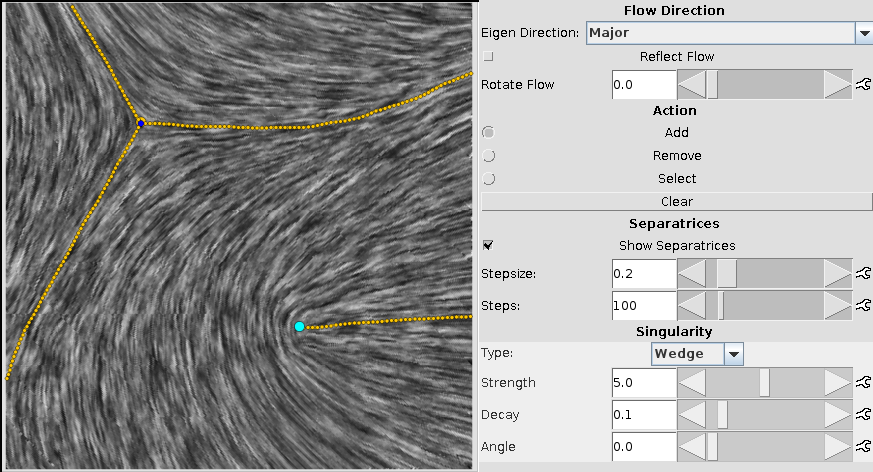
\includegraphics[scale=0.5]{img-4-2/app.png}
 \caption{Tensor Field Design Application}
 \label{fig:tfd-app}
\end{figure}

\subsection{Design Elements}

The application allows the user to interactively create a tensor field. You
choose one of six design elements (see fig. \ref{fig:tfd-elements} and
\cite{tfd}~p.~99f) and then click into the view space to place it. The
elements can be moved by drag and drop or be removed again as well.

The total second order tensor field is then defined through

\begin{equation}
 \mat{T}(\vec{r}) = \sum_i^N \mat{T}_i(\vec{r}).
 \label{eq:tf}
\end{equation}

\begin{figure}
  \centering
  \subfloat[constant]{
    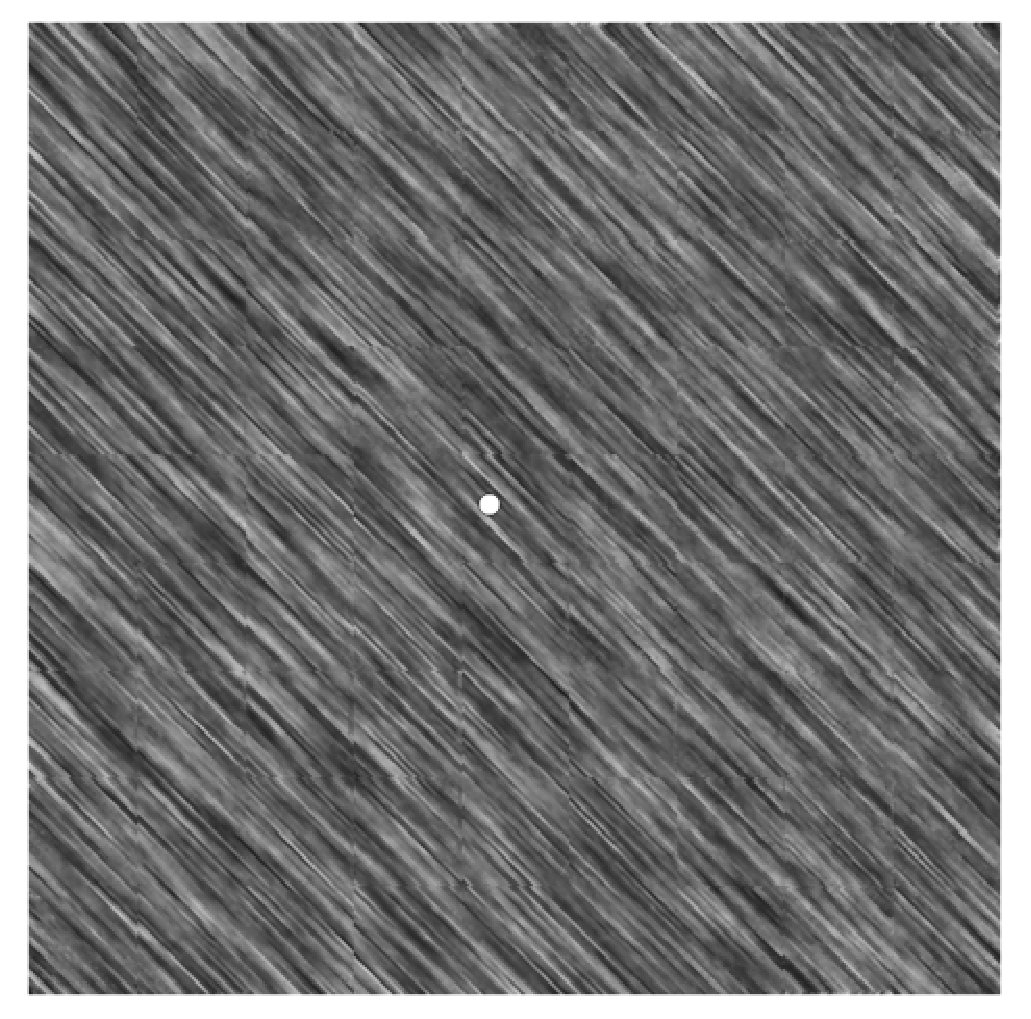
\includegraphics[width=0.3\textwidth]{img-4-2/constant.eps}}
  \subfloat[wedge]{
    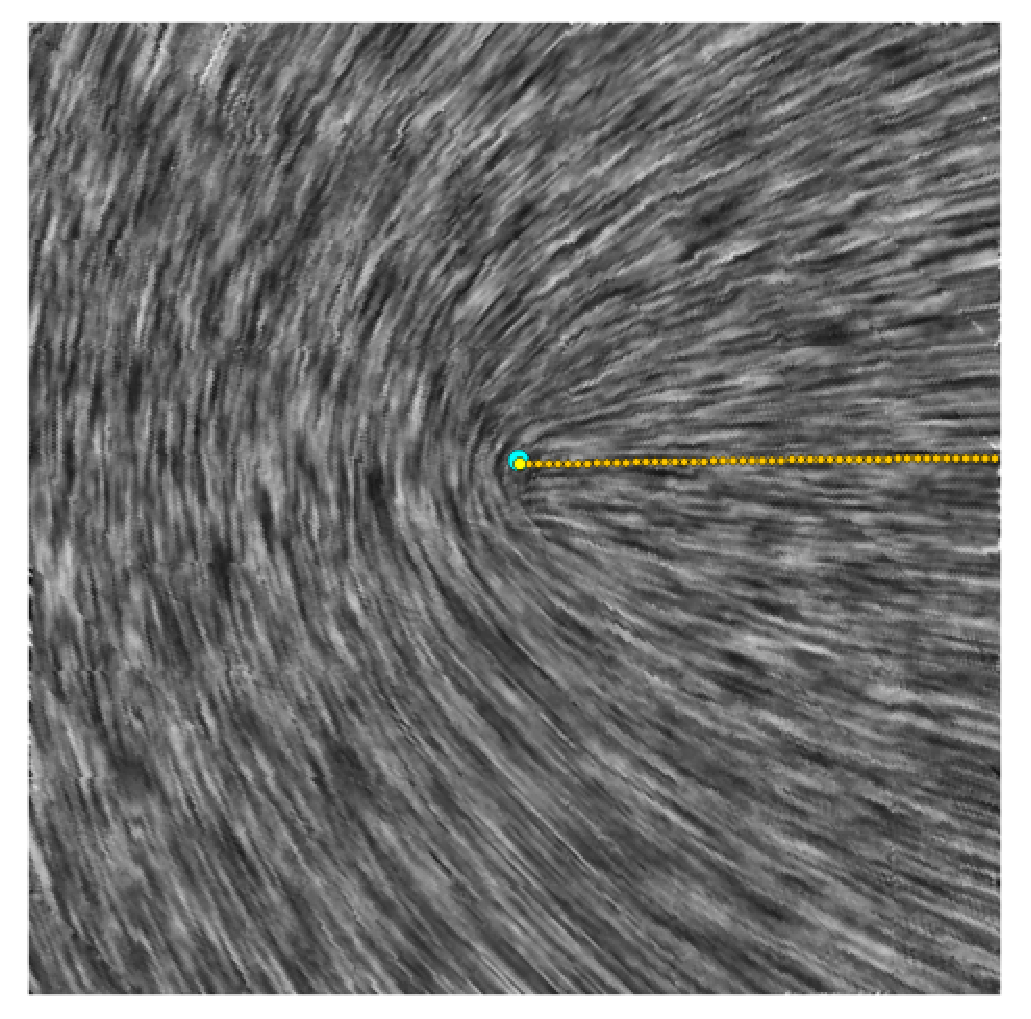
\includegraphics[width=0.3\textwidth]{img-4-2/wedge-s.eps}}
  \subfloat[trisector]{
    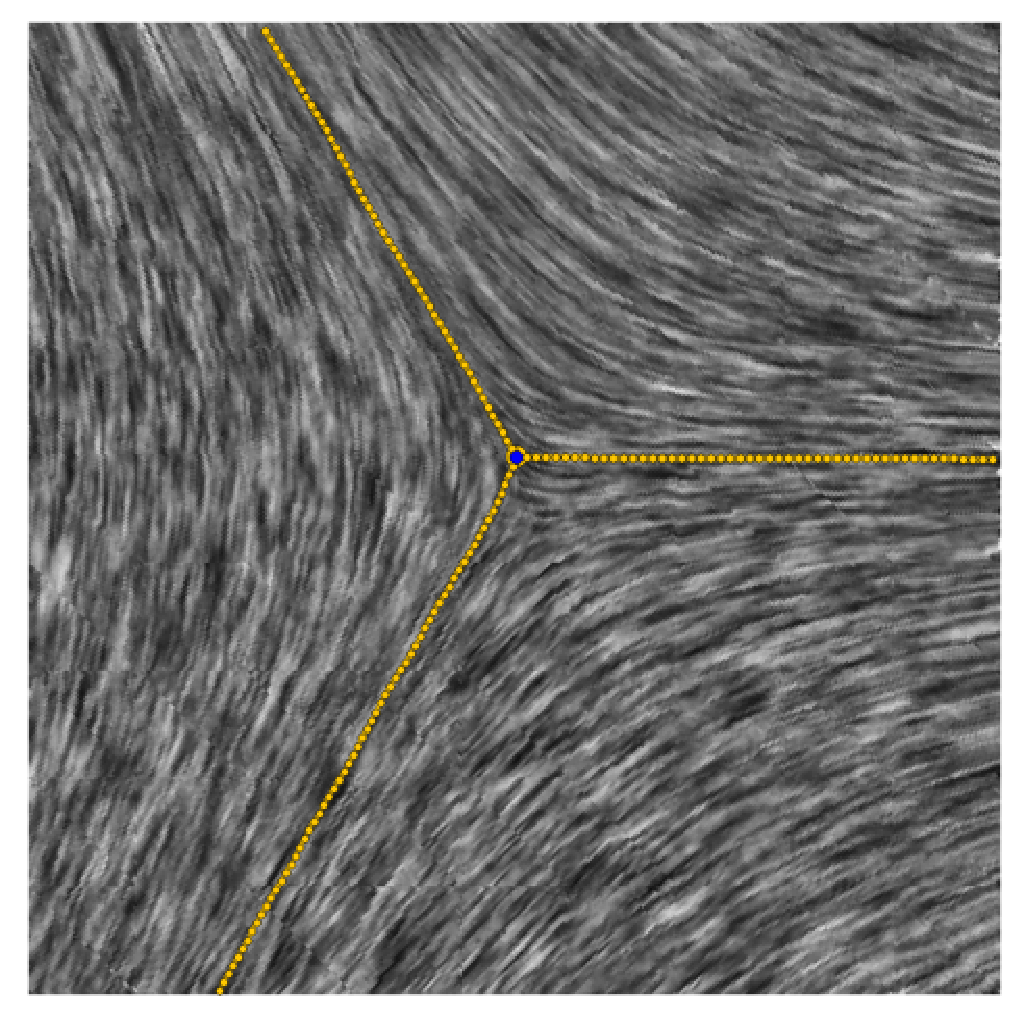
\includegraphics[width=0.3\textwidth]{img-4-2/trisector-s.eps}}
  \\
  \subfloat[node]{
    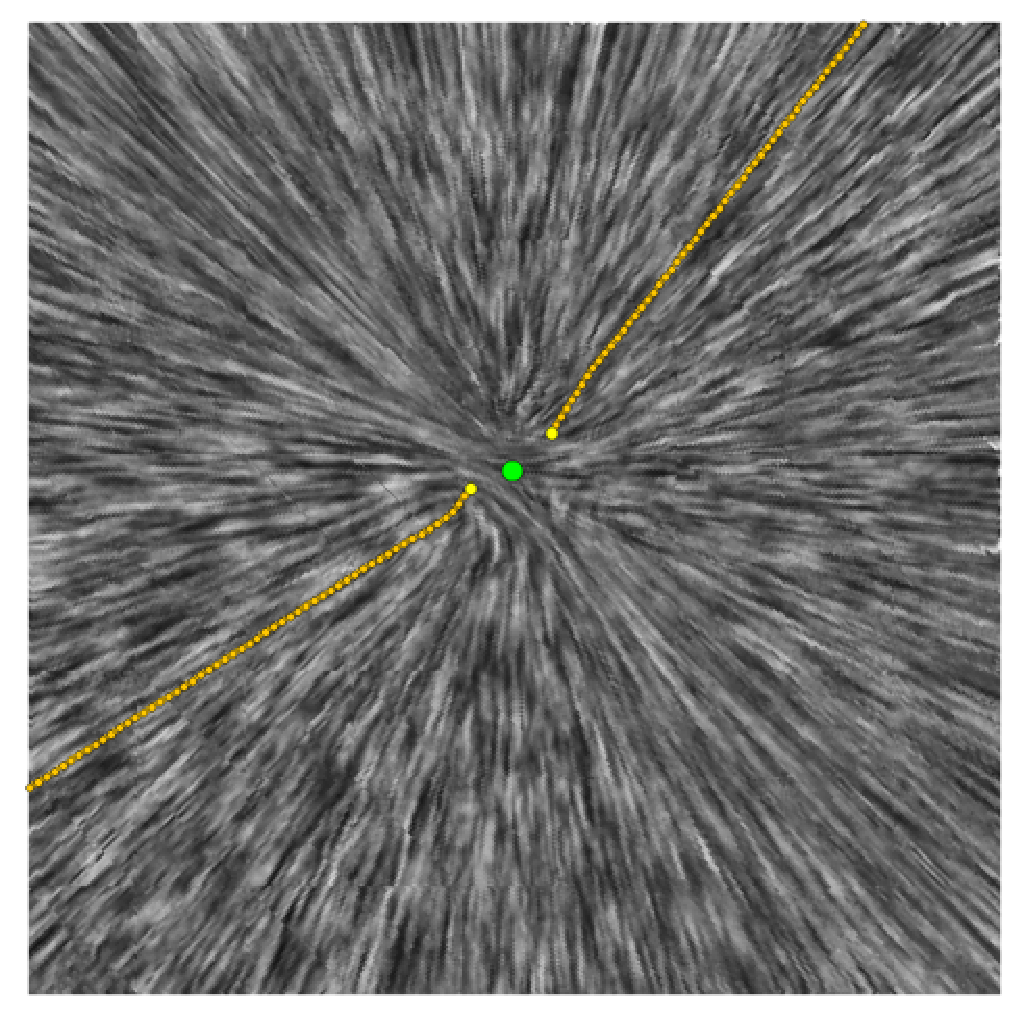
\includegraphics[width=0.3\textwidth]{img-4-2/node-s.eps}}
  \subfloat[center]{
    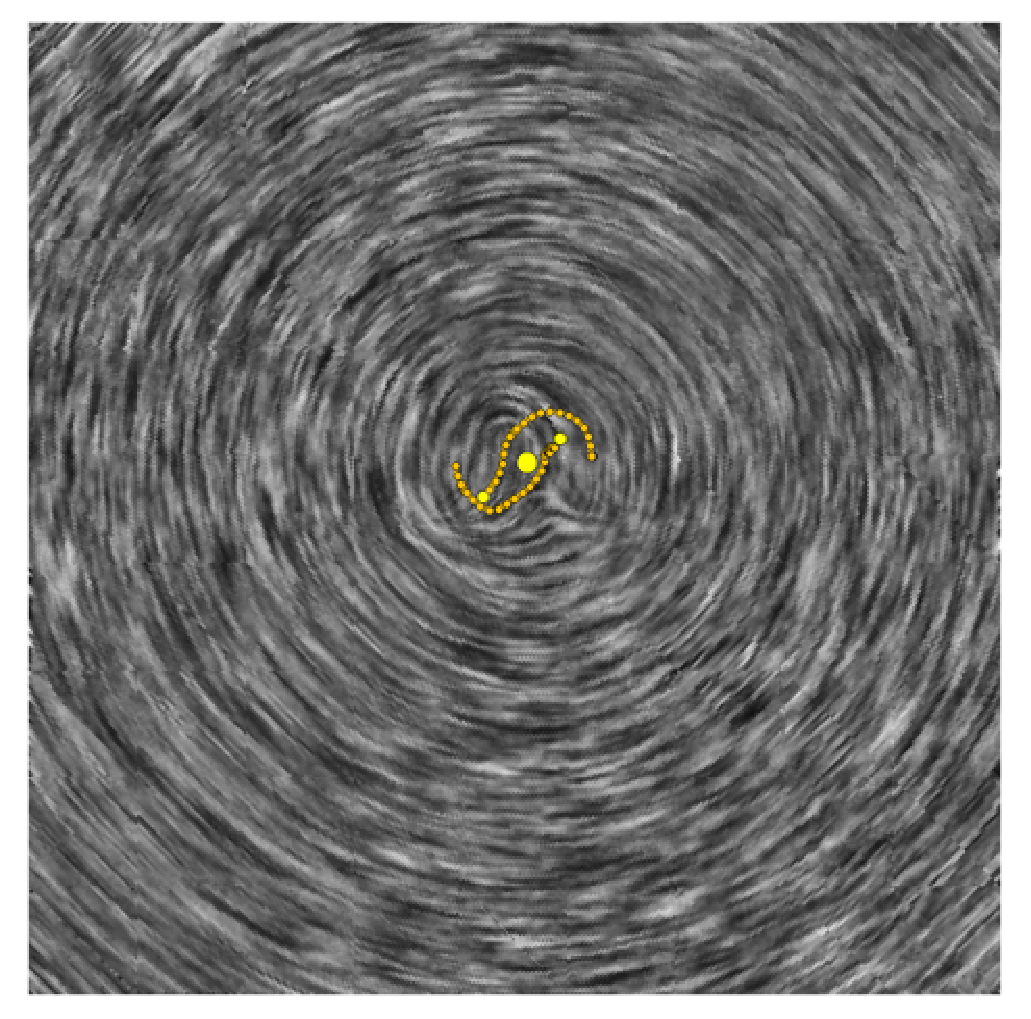
\includegraphics[width=0.3\textwidth]{img-4-2/center-s.eps}}
  \subfloat[saddle]{
    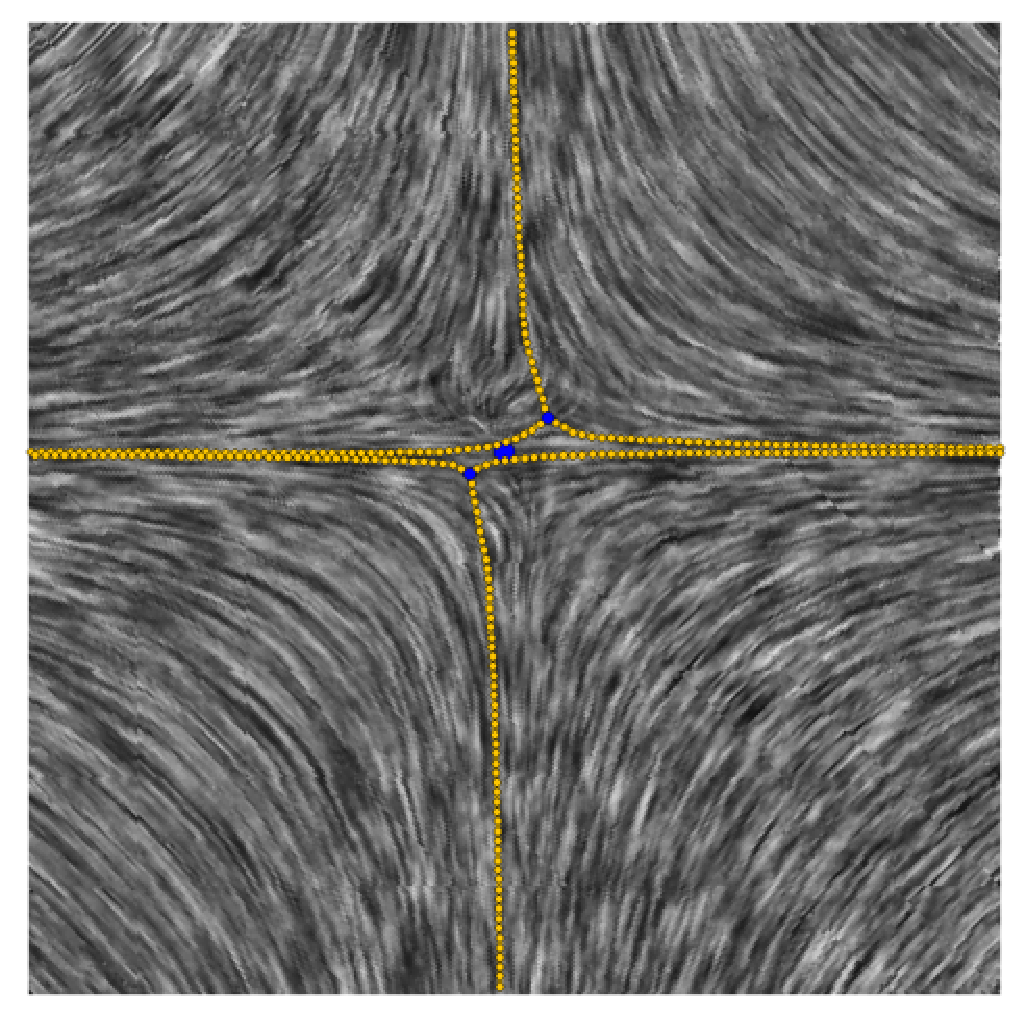
\includegraphics[width=0.3\textwidth]{img-4-2/saddle-s.eps}}
  \caption{tensor field design elements}
  \label{fig:tfd-elements}
\end{figure}

\subsection{Visualization Via Eigenvector Field}

To visualize the tensor field use the image based approach outlined in
\cite{tfd} p.~98f, which allows us to reuse the LIC code from JavaView. To
visualize the major eigenvector field, we can follow the equations outlined
there. For the minor eigenvector field though, we have to make small
adjustments: The minor eigenvector $\vec{E}_2$ is orthogonal to $\vec{E}_1$,
such that

\begin{equation}
 \vec{E}_2 = \left( \begin{array}{c}
              -\sin \theta \\
              \cos \theta
             \end{array} \right)
\end{equation}

We now create $\vec{V}_x$ such that the $x$-component is positive, i.e.:

\begin{equation}
 \vec{V}_x = \left \{  \begin{array}{l l}
                       \vec{E}_2 & \quad \text{if $-\sin \theta > 0$} \\
                       -\vec{E}_2 & \quad \text{otherwise}
                       \end{array} \right.
\end{equation}

Analogously we create $\vec{V}_y$ such that its $y$-component, i.e. $\cos
\theta$, is positive. The weighting factors $W_{x,y}$ use the $x$- and
$y$-component of $\vec{E}_2$. Hence they are

\begin{eqnarray}
 W_x &=& \sin^2 \theta \qquad \text{, and}\\
 W_y &=& 1 - W_x = \cos^2 \theta .
\end{eqnarray}

You can see an example of the above code in fig. \ref{fig:tfd-majorminor}.

\begin{figure}
  \centering
  \subfloat[major]{
    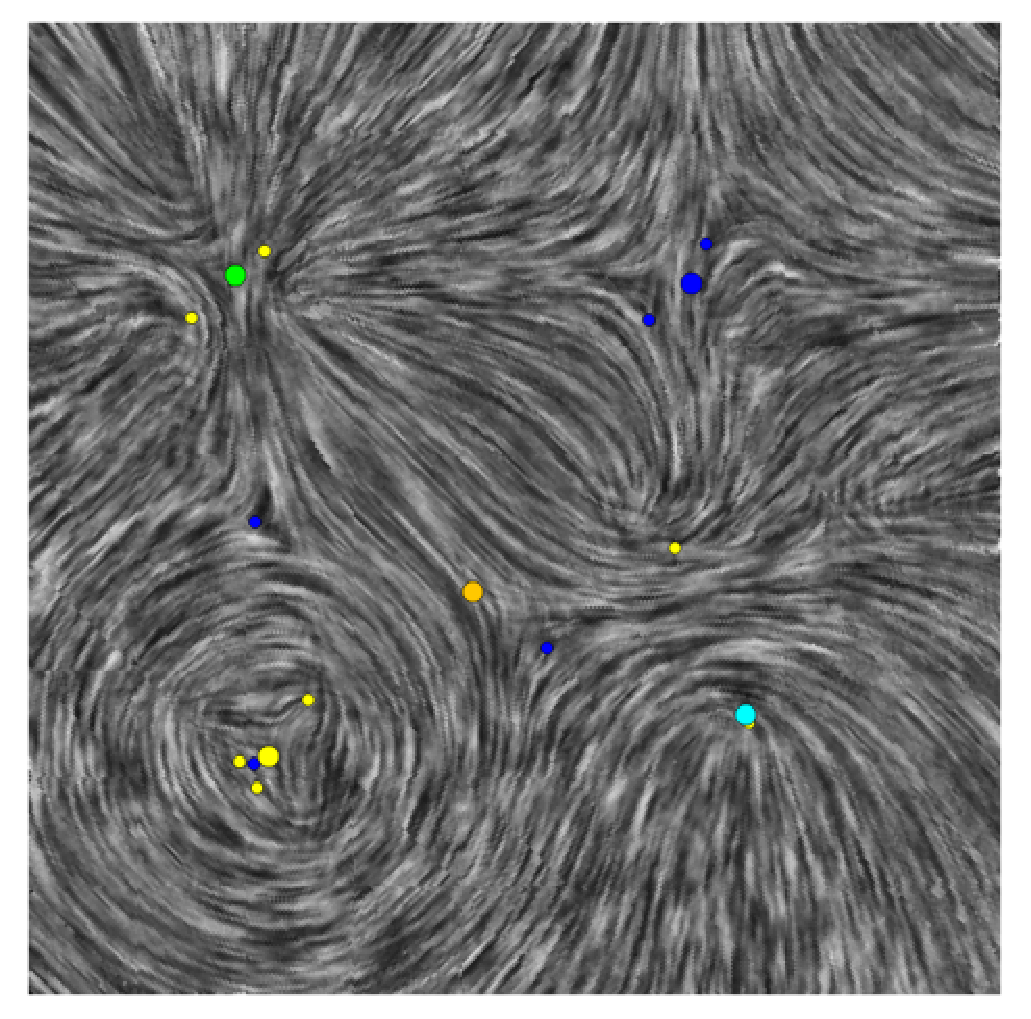
\includegraphics[width=0.4\textwidth]{img-4-2/major.eps}
    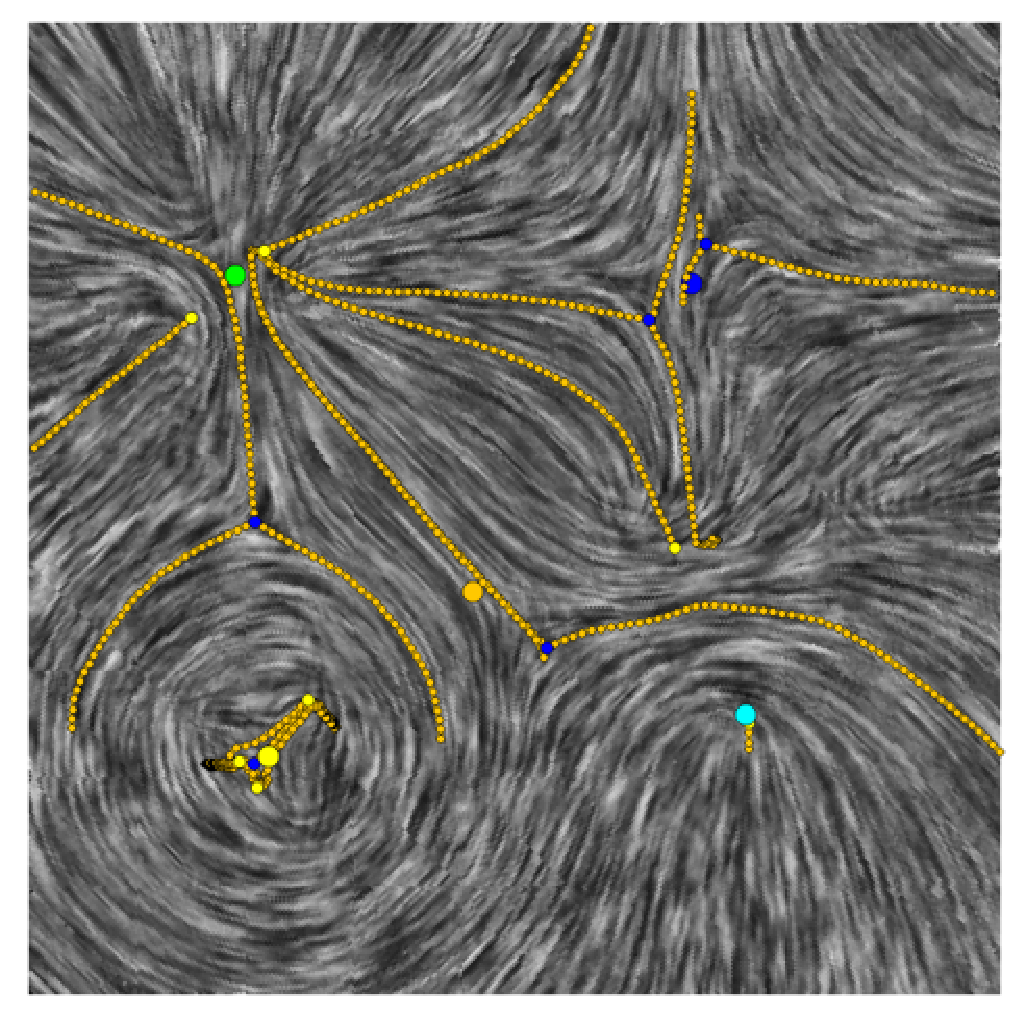
\includegraphics[width=0.4\textwidth]{img-4-2/major-s.eps}
  }
  \\
  \subfloat[minor]{
    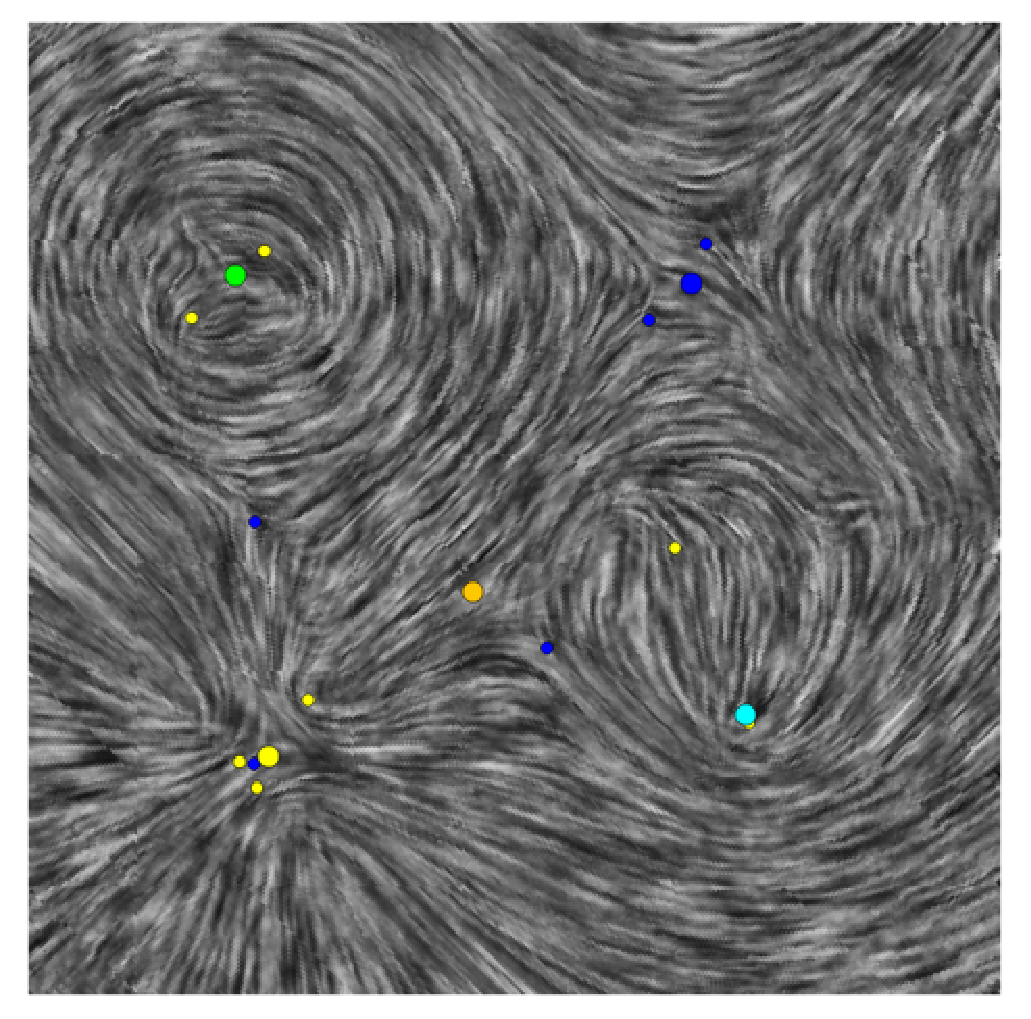
\includegraphics[width=0.4\textwidth]{img-4-2/minor.eps}
    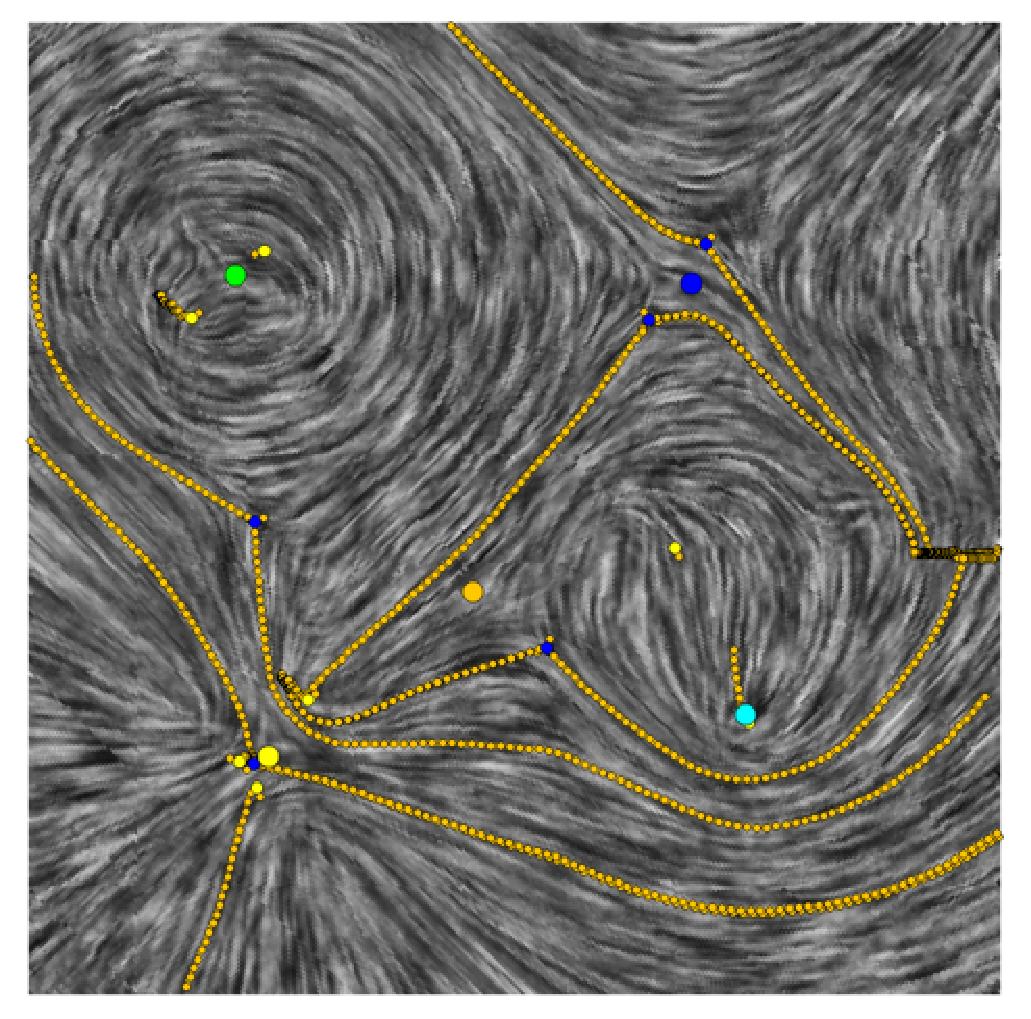
\includegraphics[width=0.4\textwidth]{img-4-2/minor-s.eps}
  }
  \caption{minor and major eigenvector fields}
  \label{fig:tfd-majorminor}
\end{figure}

\subsection{Rotation and Reflection}

To rotate the tensor field by an angle $\theta$, we use the reflection matrix

\begin{equation}
 \mat{R} = \left( \begin{array}{cc}
            \cos(\theta/2) & -\sin(\theta/2) \\
            \sin(\theta/2) & \cos(\theta/2) \end{array}
\right)
\end{equation}

The rotated tensor field is then obtained from eq. \ref{eq:tf} using

\begin{equation}
 \mat{T}'(\vec{r}) = \mat{R} \mat{T}(\vec{r}) \mat{R}^T.
\end{equation}

To additionally reflect the tensor field along the axis defined by $\theta$, we
can use a reflection matrix $\mat{R}'$ instead of $\mat{R}$:

\begin{equation}
 \mat{R}' = \left( \begin{array}{cc}
            \cos(\theta/2) & \sin(\theta/2) \\
            \sin(\theta/2) & -\cos(\theta/2) \end{array}
\right)
\end{equation}

Take a look at fig. \ref{fig:tfd-rotation} for tensor field rotation and at
fig. \ref{fig:tfd-reflection} for tensor field reflection.

\begin{figure}
  \centering
  \subfloat[original]{
    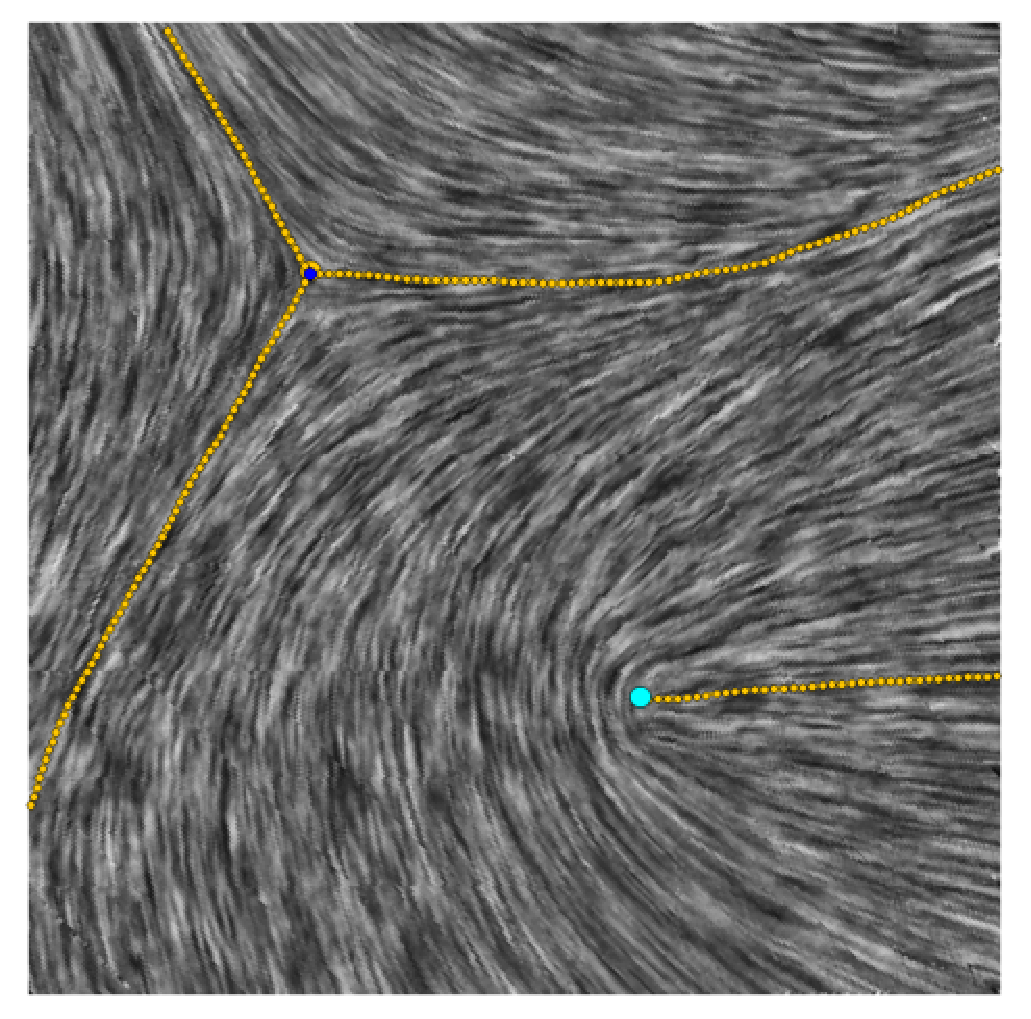
\includegraphics[width=0.3\textwidth]{img-4-2/wedge-trisector-base.eps}}
  \subfloat[$45\degree$]{
    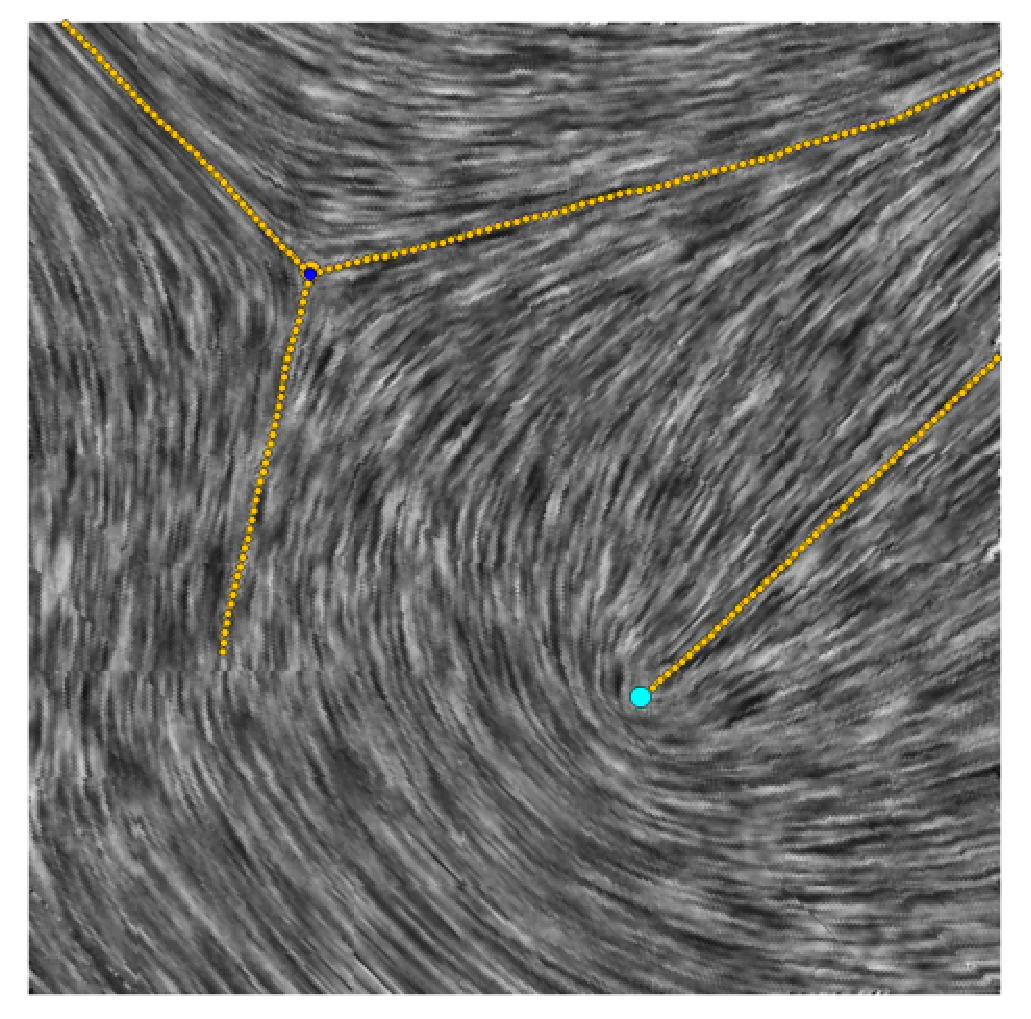
\includegraphics[width=0.3\textwidth]{img-4-2/wedge-trisector-45.eps}}
  \subfloat[$90\degree$]{
    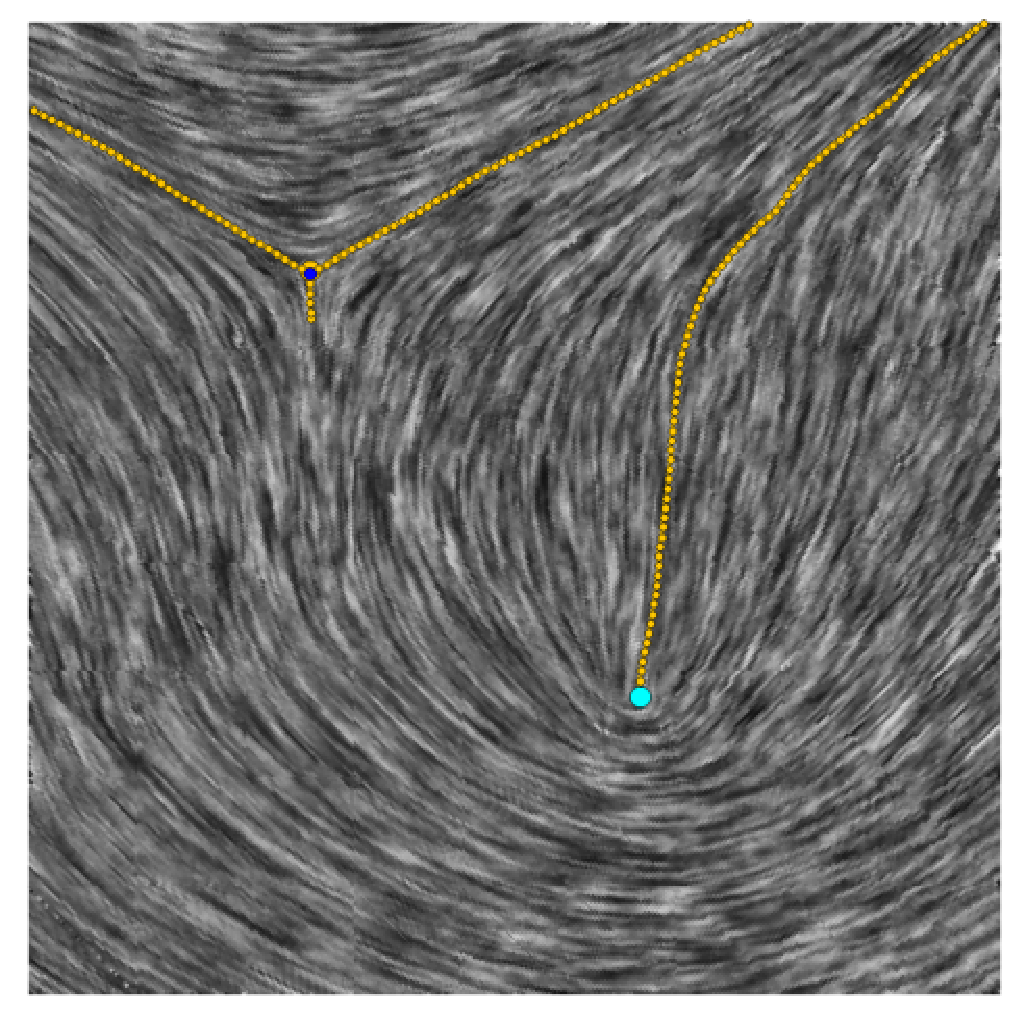
\includegraphics[width=0.3\textwidth]{img-4-2/wedge-trisector-90.eps}}
  \\
  \subfloat[$135\degree$]{
    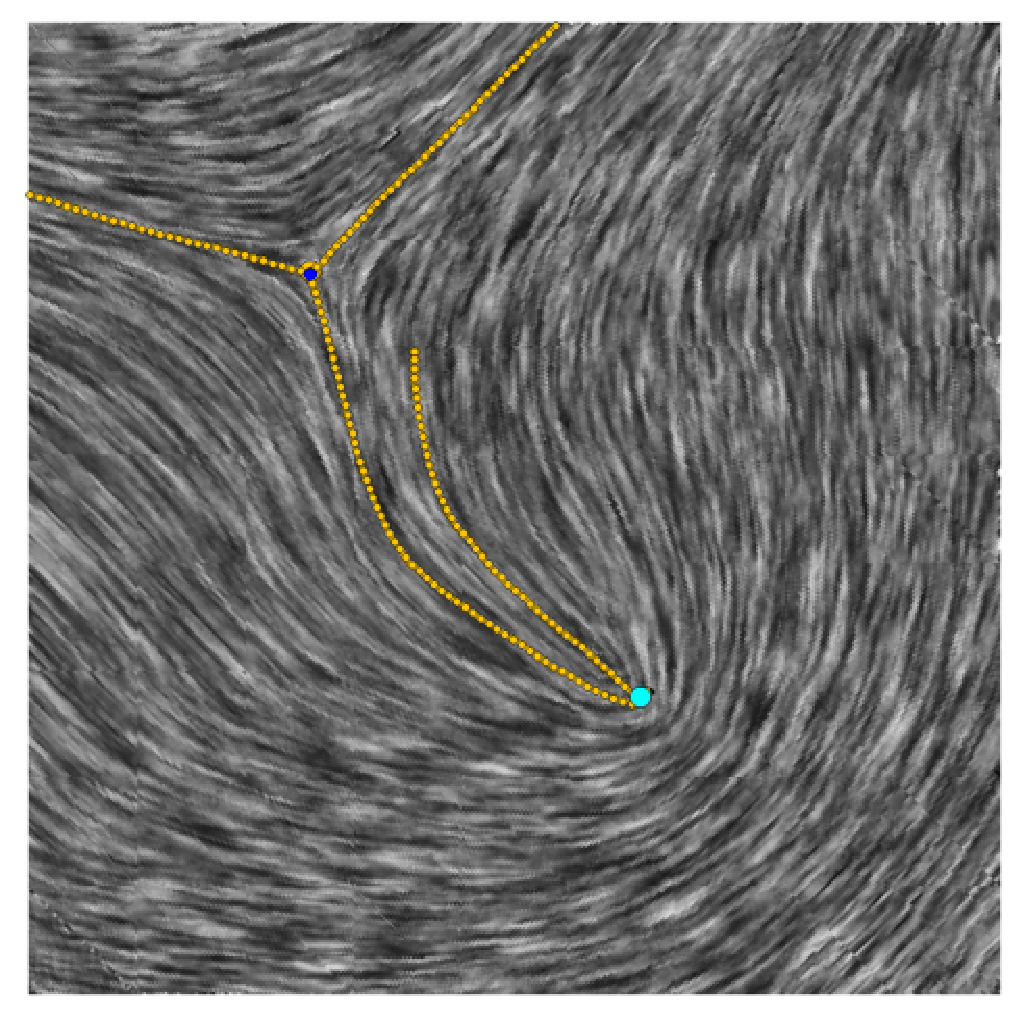
\includegraphics[width=0.3\textwidth]{img-4-2/wedge-trisector-135.eps}}
  \subfloat[$180\degree$]{
    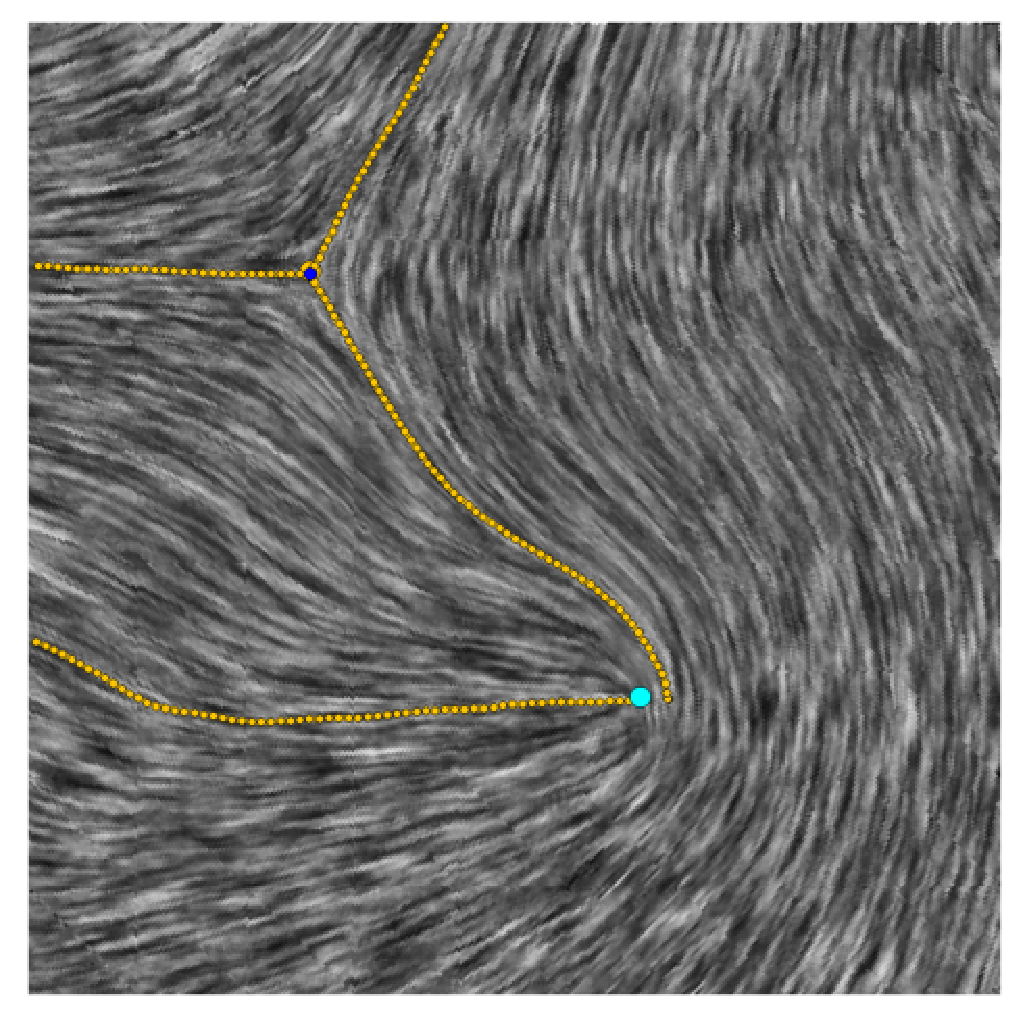
\includegraphics[width=0.3\textwidth]{img-4-2/wedge-trisector-180.eps}}
  \subfloat[$270\degree$]{
    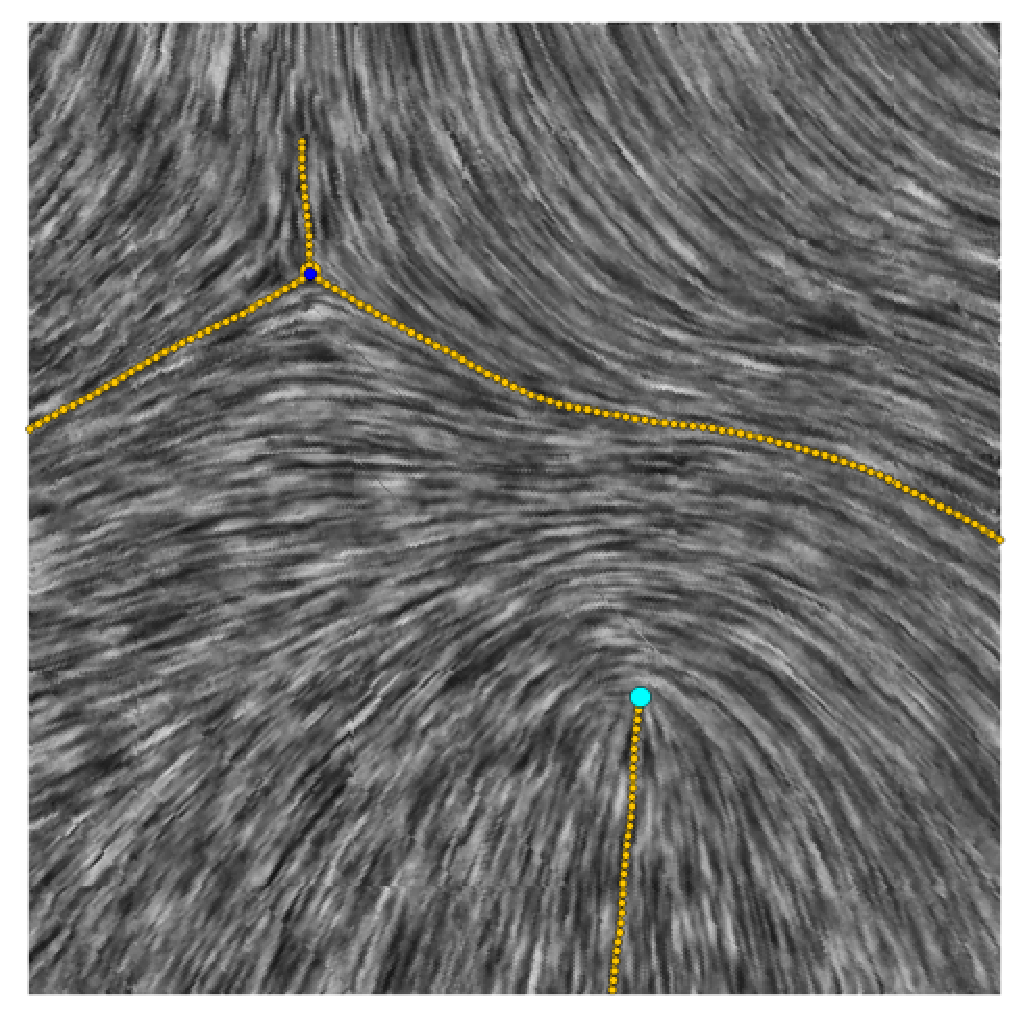
\includegraphics[width=0.3\textwidth]{img-4-2/wedge-trisector-270.eps}}
  \caption{tensor field rotation}
  \label{fig:tfd-rotation}
\end{figure}

\begin{figure}
  \centering
  \subfloat[original]{
    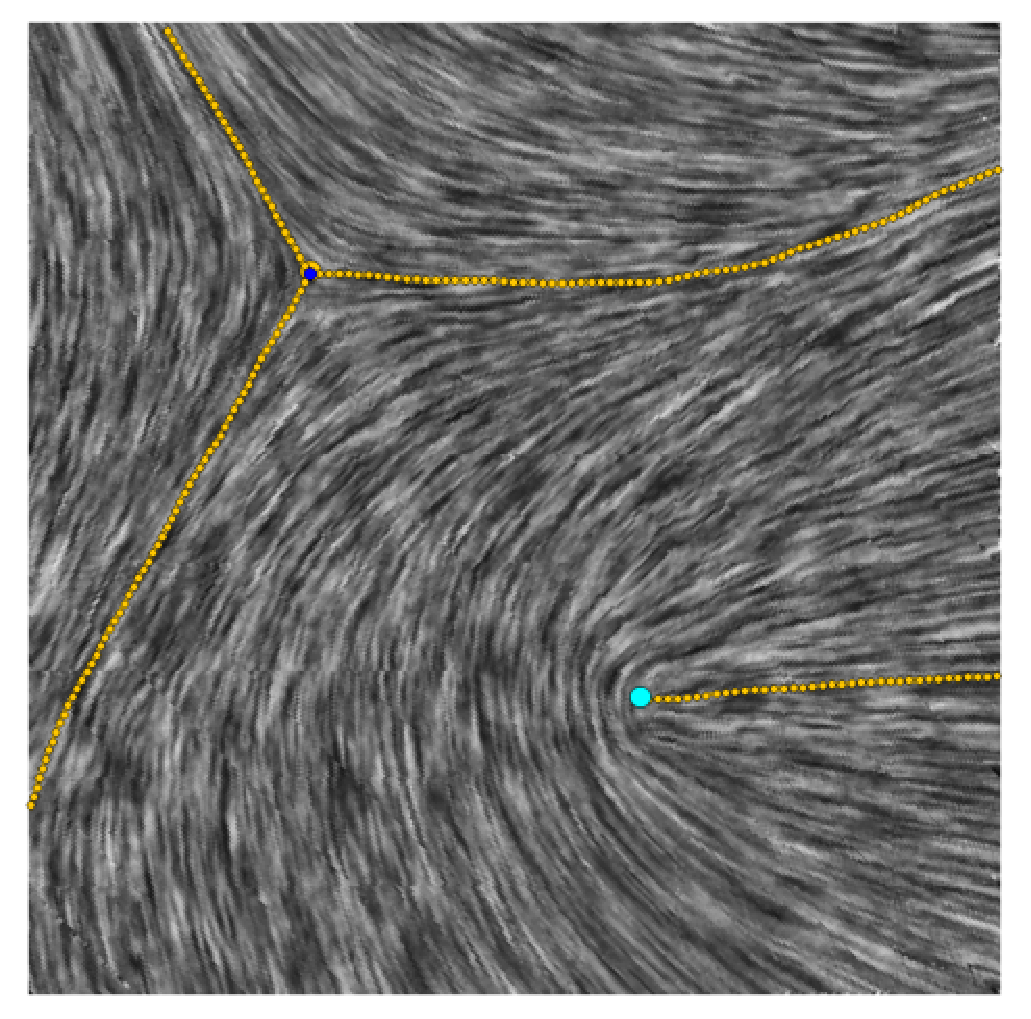
\includegraphics[width=0.4\textwidth]{img-4-2/wedge-trisector-base.eps}}
  \subfloat[reflected]{
    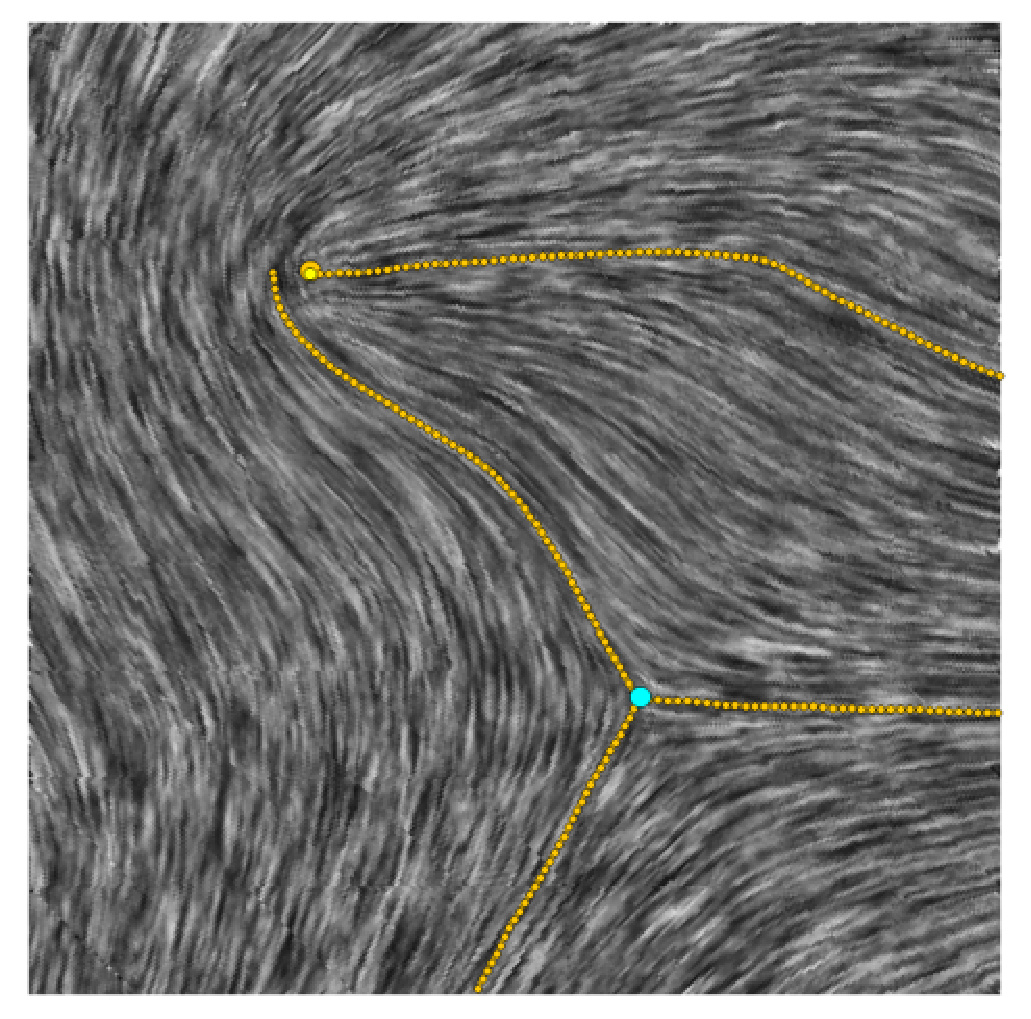
\includegraphics[width=0.4\textwidth]{img-4-2/wedge-trisector-reflect.eps}
  }
  \caption{tensor field reflection}
  \label{fig:tfd-reflection}
\end{figure}


\bibliography{sources}

\end{document}

% kate: replace-tabs on;